\section*{集合}\label{sec:Collection}



\subsection*{集合的特点}
数组可以存储基本数据类型和引用数据类型。集合只能存储引用数据类型,存储基本数据类型会报错。但是可以把基本数据类型改为包装类数据来放入集合。
\lstinputlisting[style=Java]{../../../Collection/src/com/learnjava/collection/CollectionDemo1.java}

还有数组的长度是固定的,但是集合的长度是可以改变的。

\subsection*{集合的体系结构}

\begin{figure}
    \centering
    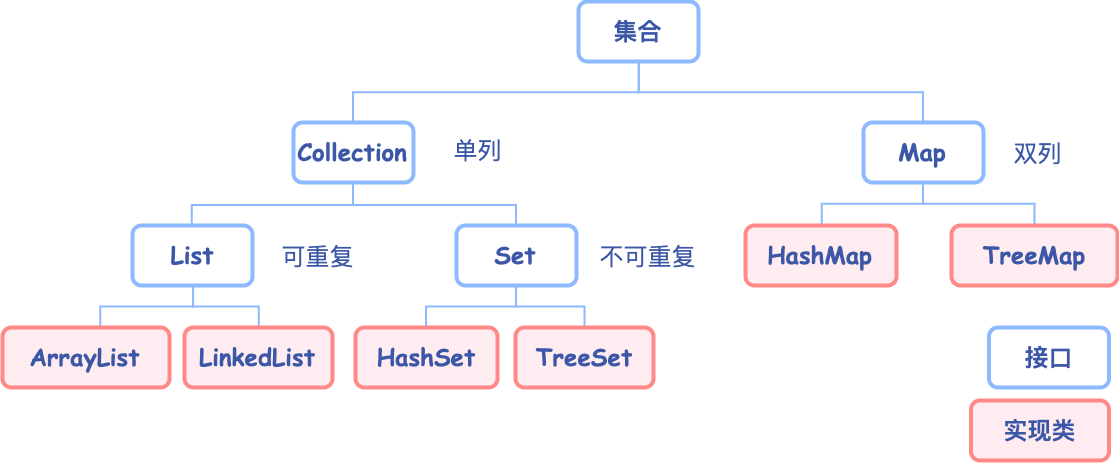
\includegraphics[width=.7\textwidth]{img/collection/1.png}
 %   \caption{best} %caption是图片的标题
\end{figure}



如果数据是单个的数据集合,就是单列数据结构,称之为Collection。如果是以键值对的方式存在的集合,称之为Map。

List和Set都是接口,实际的List和Set指的都是它们的实现类。List的实现类有ArryList、LinkedList。Set的实现类有HashSet、TreeSet。
Map也是接口,实际的Map指是的它的实现类。Map的实现类有HashMap、TreeMap。

\subsection*{集合常用的方法}
collection是一个接口,new的时候要new实现对象。这是多态的表现。具体请查看多态章节。
\begin{lstlisting}[style=Java]
Collection<String> collection = new ArrayList<>();
\end{lstlisting}

\subsubsection*{add,remove}
\lstinputlisting[
    style=Java,
    linerange={5-22}
]{../../../Collection/src/com/learnjava/collection/CollectionDemo2.java}

\subsubsection*{removeif}
可以传入lambda表达式。lambda表达式为remove的过滤条件。
\lstinputlisting[
    style=Java,
    linerange={6-23}
]{../../../Collection/src/com/learnjava/collection/CollectionDemo3.java}

传入的lambda表达式,s表示集合中的每一个元素。每一个元素都会到return的表达式中判断一下,如果返回的是true就保留,如果返回的是false就删除。

为什么会传入一个lambda表达式呢?点进removeIf的源码:

\begin{lstlisting}[style=Java]
    default boolean removeIf(Predicate<? super E> filter) {
\end{lstlisting}

removeIf需要传入的是一个符合Predicate接口的对象作为参数。Predicate也是函数式接口,因此可以使用Lambda表达式。

从Predicate接口的代码中可以看到,其本身是一个接口,里面只有一个test(T t)的抽象方法。对t进行断言,返回true或者false。

\begin{lstlisting}[style=Java]
    public interface Predicate<T> {
        /**
            * Evaluates this predicate on the given argument.
            *
            * @param t the input argument
            * @return {@code true} if the input argument matches the predicate,
            * otherwise {@code false}
            */
        boolean test(T t);
        ...
\end{lstlisting}



